\section{Observatorio Astronómico Universitario - Iturbide} \label{muestra:observaciones:oau}

El \textbf{Observatorio Astronómico Universitario - Iturbide} (el cual de ahora
en adelante será referido como el OAU), ubicado en el cerro Picacho en el
municipio de Iturbide, Nuevo León, es un nuevo sitio dedicado a la observación
astronómica, equipado para realizar observaciones del Sol, monitoreo de basura
espacial, y la observación de objetos variables, como los sistemas binarios o
asteroides. A continuación se describe el equipo utilizado; como software de
control se utilizó \textbf{Nighttime Imaging 'N'
Astronomy}\footnote{\myurl{https://nighttime-imaging.eu}} (\textbf{NINA}), el cual
permita consolidar el control de todas las componentes mecánicas en una sola
aplicación. 

% TODO: look for mount documentation
El telescopio utilizado para hacer las observaciones del sistema fue el tubo
óptico \textbf{CDK20} de \textbf{PlaneWave
Instruments}\footnote{\myurl{https://planewave.com/product/cdk20-ota/}} con un
número $f/6.8$. Este telescopio de diseño \textit{Dall-Kirkham corregido} cuenta
con un grupo de lentes frente al espejo esférico secundario, el cual resta los
efectos de la aberración esférica presente en otras configuraciones de espejos
primarios y secundarios, resultando en una imagen más nítida. Este instrumento,
combinado con una montura ecuatorial \textbf{Orion HDX110}, nos permite una
vista clara de la bóveda celeste a \ang{30} arriba del horizonte, con capacidad
de observar objetos tenues más allá de 17 magnitudes.

El CCD usado para obtener las imágenes fue el
\textbf{QHY174GPS}\footnote{\myurl{https://www.qhyccd.com/qhy174gps-imx174-scientific-cooled-camera/}}.
Este CCD cuenta con una resolución de $1920 \times 1200$ pixeles. Para reducir
el ruido térmico tiene un mecanismo de enfriamiento termoeléctrico, el cual lo
puede enfriar a una temperatura de -\ang{40} C bajo la temperatura ambiente.
Frente al CCD va equipado una rueda de filtros \textbf{ZWO
7x36mm}\footnote{\myurl{https://astronomy-imaging-camera.com/product/new-zwo-efw-7x36mm/}},
la cual puede ser equipada con 7 filtros distintos. Para las observaciones
recabadas en este trabajo, utilizamos solamente el filtro \textbf{Luminance}, el
cual se aproxima a la región del visible del espectro electromagnético
(\reffigure{zwoFilterTransmissionCurve}, obtenida de la página comercial de
ZWO\footnote{\url{https://astronomy-imaging-camera.com/product/zwo-lrgb-36mm-filters/}}). 

\begin{figure}[!ht]
	\centering
	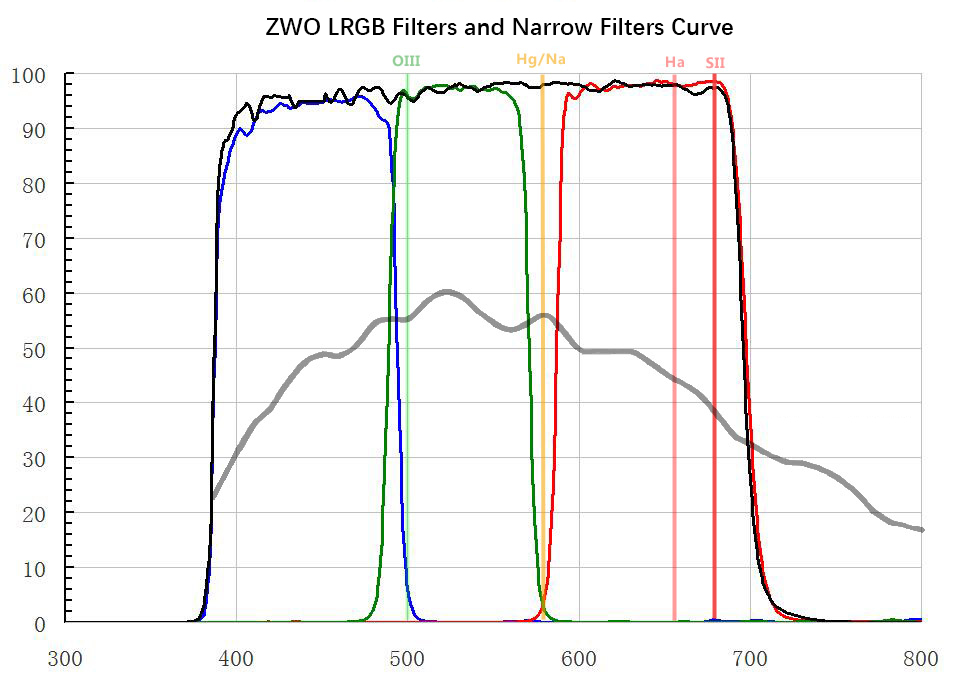
\includegraphics[scale=0.6]{Observaciones/Secciones/Figures/ZWO RGBL Transmission Curve.jpg}
	\caption{Curva de transmisión de filtros de ZWO. El filtro de
	\textbf{Luminance} se encuentra como la curva negra, abarcando todo el
	espectro visible, desde los 400nm hasta 700nm. Gráfica obtenida de la
	página de productos de ZWO.}
	\label{zwoFilterTransmissionCurve}
\end{figure}